\chapter{Discussion}
Please tell more about conclusion and how to the next work of this study.

\section{Imron Sumadireja / 1164076}
\subsection{Teori}
\begin{enumerate}
\item Jelaskan kenapa file teks harus dilakukan tokenizer. Dilengkapi dengan ilustrasi atau gambar \par
Tokenizer merupakan proses membagi teks yang dapat berupa kalimat, paragraf atau dokumen menjadi kata-kata atau bagian-bagian tertentu dalam kalimat tersebut. Sebagai contoh dari kalimat `Aku mau istirahat dulu ya untuk hari ini', menjadi `Aku', `Mau', `'Istirahat',`Dulu',`Ya',`Untuk',`Hari',`Ini'. Yang menjadi acuan yakni tanda baca dan spasi. Untuk ilustrasinya bisa dilihat pada gambar \ref{toke1}
		\begin{figure}[!htbp]
		\centerline{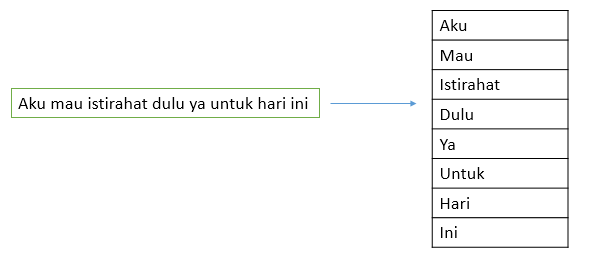
\includegraphics[width=0.5\textwidth]{figures/im/toke1.png}}
		\caption{Ilustrasi Tokenizer.}
		\label{toke1}
		\end{figure}

\item Jelaskan konsep dasar K Fold Cross Validation pada dataset komentar Youtube pada kode listing 7.1.dilengkapi dengan ilustrasi atau gambar \par
\begin{verbatim}
kfold = StratifiedKFold(n_splits=5)
splits = kfold.split(d, d['CLASS'])
\end{verbatim}
Pada code tesebut terdapat kfold yang bertujuan untuk melakukan split data menjadi 5 bagian dari dataset komentar Youtube tersebut. Sehingga dari setiap data yang sudah dibagi tersebut akan menghasilkan presentase dari setiap bagiannya, untuk menghasilkan hasil akhir dengan presentase yang cukup baik. Untuk ilustrasi sederhananya bisa dilihat pada gambar \ref{toke2}
		\begin{figure}[!htbp]
		\centerline{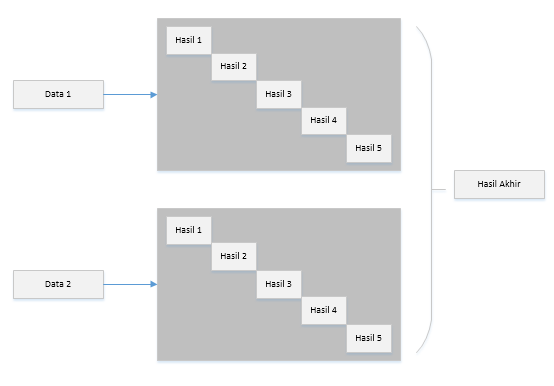
\includegraphics[width=0.5\textwidth]{figures/im/toke2.png}}
		\caption{Ilustrasi K-Fold Cross Validation.}
		\label{toke2}
		\end{figure}

\item Jelaskan apa maksudnya kode program for train, test in splits. Dilengkapi dengan ilustrasi atau gambar \par
For train ini untuk membagi data tersebut menjadi data training. Sedangkan test in splits ini untuk menguji apakah dataset tersebut sudah dibagi menjadi beberapa bagian atau masih menumpuk. Untuk ilustrasi sederhananya bisa dilihat pada gambar \ref{toke3}
		\begin{figure}[!htbp]
		\centerline{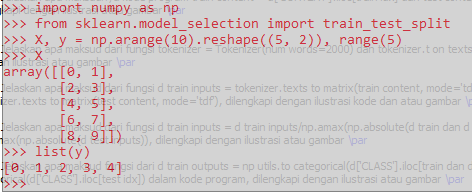
\includegraphics[width=0.5\textwidth]{figures/im/toke3.png}}
		\caption{For Train dan Test In Splits.}
		\label{toke3}
		\end{figure}

\item Jelaskan apa maksudnya kode program train content = d['CONTENT'].iloc[train idx] dan test content = d['CONTENT'].iloc[test idx]. dilengkapi dengan ilustrasi atau gambar \par
Code tersebut untuk mengambil data pada kolom atau index CONTENT yang merupakan bagian dari train\_idx dan test\_idx. Contoh sederhananya ketika data telah diubah menjadi data train dan data test maka kita dapat memilihnya untuk ditampilkan pada kolom yang diinginkan. Untuk ilustrasinya bisa dilihat pada gambar \ref{toke4}
		\begin{figure}[!htbp]
		\centerline{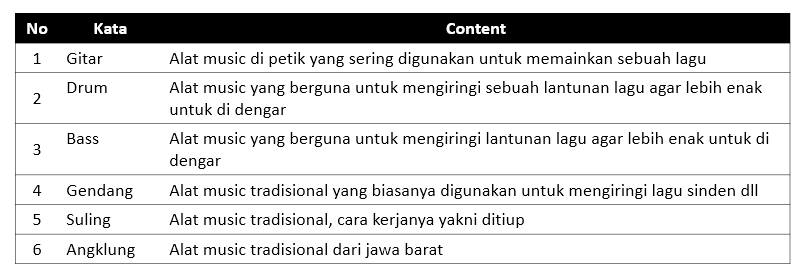
\includegraphics[width=0.5\textwidth]{figures/im/toke4.png}}
		\caption{Ilustrasi Content.}
		\label{toke4}
		\end{figure}

\item Jelaskan apa maksud dari fungsi tokenizer = Tokenizer(num words=2000) dan tokenizer.fit on texts(train content), dilengkapi dengan ilustrasi atau gambar \par
Variabel tokenizer ini berfungsi untuk melakukan vektorisasi data kedalam bentuk token sebanyak 2000 kata. Dan selanjutnya akan melakukan fit tokenizer hanya untuk data training saja tidak dengan data testingnya. Untuk ilustrasinya bisa dilihat pada gambar 

\item Jelaskan apa maksud dari fungsi d train inputs = tokenizer.texts to matrix(train content, mode='tdf') dan d test inputs = tokenizer.texts to matrix(test content, mode='tdf'), dilengkapi dengan ilustrasi kode dan atau gambar \par

\item Jelaskan apa maksud dari fungsi d train inputs = d train inputs/np.amax(np.absolute(d train dan d test inputs = d test inputs/np.amax(np.absolute(d test inputs)), dilengkapi dengan ilustrasi atau gambar \par

\item Jelaskan apa maksud fungsi dari d train outputs = np utils.to categorical(d['CLASS'].iloc[train dan d test outputs = np utils.to categorical(d['CLASS'].iloc[test idx]) dalam kode program, dilengkapi dengan ilustrasi atau gambar \par

\item Jelaskan apa maksud dari fungsi di listing 7.2. Gambarkan ilustrasi Neural Network nya dari model kode tersebut \par

\item Jelaskan apa maksud dari fungsi di listing 7.3 dengan parameter tersebut \par

\item Jelaskan apa itu Deep Learning \par
Deep Learning adalah salah satu cabang dari ilmu machine learning yang terdiri dari algoritma pemodelan abstraksi tingkat tinggi pada data menggunakan sekumpulan fungsi transformasi non-linear yang ditata berlapis-lapis dan mendalam. Teknik dan algoritma dalam machine learning dapat digunakan baik untuk supervised learning dan unsupervised learning.

\item Jelaskan apa itu Deep Neural Network, dan apa bedanya dengan Deep Learning \par
DNN adalah salah satu algoritma berbasis jaringan saraf tiruan yang memiliki dari 1 lapisan saraf tersembunyi yang dapat digunakan untuk pengambilan keputun. Perbedaannya dengan deep learning, yakni: DNN dapat menentukan dan mencerna karakteristik tertentu di suatu rangkaian data, kapabilitas lebih kompleks untuk mempelajari, mencerna, dan mengklasifikasikan data, serta dibagi ke dalam berbagai lapisan dengan fungsi yang berbeda-beda.

\item Jelaskan dengan ilustrasi gambar buatan sendiri(langkah per langkah) bagaimana perhitungan algoritma konvolusi dengan ukuran stride (NPM mod3+1) x (NPM mod3+1) yang terdapat max pooling \par

\end{enumerate}

\section{Yusniar Nur Syarif Sidiq / 1164089}
\subsection{Teori / Yusniar Nur Syarif Sidiq / 1164089}
\begin{enumerate}

\item Jelaskan kenapa file teks harus di lakukan tokenizer. Dilengkapi dengan ilustrasi atau gambar !
	\subitem Sebelumnya kita harus tau terlebih dahulu apa itu Tokenizer, yaitu sebuah proses pembagian terhadap kalimat yang berada dalam dokumen sehingga menjadi sebuah bagian - bagian kata atau bisa kita sebut denga token. Dalam dataset Youtube Tokenizer digunakan untuk melakukan vektorisasi data, sehingga dapat kita simpulkan bahwa data yang telah kita buat dokumen pada chapter 6 yaitu data spam dan bukan spam akan dilakukan vektorisasi dengan menggunakan Tokenizer ini. Ilustrasi sederhana mengenai Tokenizer ini misalkan saya memiliki sebuah kalimat Nama Saya Adalah Yusniar jika gunakan fungsi Tokenizer ini akan dipecah menjadi kata per kata, perhatikan figure \ref{YNC7-1}.

	\begin{figure}[!htbp!]
		\centerline{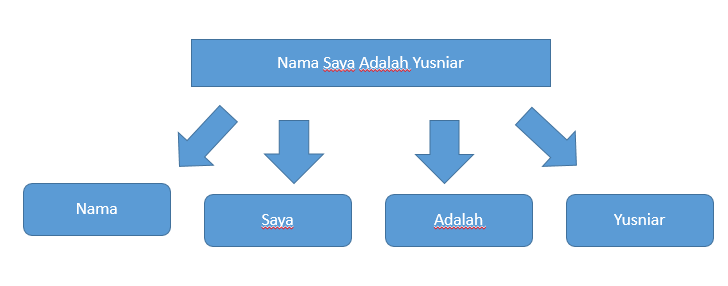
\includegraphics[width=0.5\textwidth]{figures/YN/Chapter7/YNC7-1.png}}
		\caption{Contoh Tokenizer.}
		\label{YNC7-1}
	\end{figure}

\item Jelaskan konsep dasar K Fold Cross Validation pada dataset komentar Youtube pada source code dibawah. Dilengkapi dengan ilustrasi atau gambar !

	\begin{verbatim}
		k f o l d = S t r a t i f i e d K F o l d ( n s p l i t s =5)
		2 s p l i t s = k f o l d . s p l i t ( d , d ['CLASS'] )
	\end{verbatim}

	\subitem Pada variabel kfold berisikan StratifieldKFold yang dimana akan diisikan sebuah sempel dan dibagi menjadi 5 dengan nsplits pada setiap class. Lalu akan dibuat variabel baru yang dinamakan dengan 2splits dan disikan class dari dataset Youtube.

\item Jelaskan apa maksudnya kode program for train, test in splits. Dilengkapi dengan ilustrasi atau gambar !
	\subitem Dimana fungsi tersebut digunakan untuk melakukan pengujian terhadap data yang sudah di split atau belum dalam dataset dan tidak akan terjadi penumpukan, maksudnya pada setiap class tidak akan menampilkan id yang sama. Kali ini saya akan memberikan ilustrasi sederhana, misalkan ada seseorang yang ingin menyumbangkan buku cerita kepada perpustakan, lalu pihak perpustakaan akan menerimanya, dikarenakan yang di sumbangkan adalah buku cerita dan bermacam - macam maka tidak akan ada buku yang sama hal ini sama saja bisa dibilang tidak adanya id yang sama.

\item Jelaskan apa yang dimaksud kode program dibawah. Dilengkapi dengan ilustrasi atau gambar !
	
	\begin{verbatim}
	#1
	train content = d['CONTENT'].iloc[train idx]
	#2
	test content = d['CONTENT'].iloc[test idx]
	\end{verbatim}

	\subitem Dimana source code tersebut akan mengambil data dari kolom Content yaitu kolom tersebut merupakan bagian dari train\_idx dan test\_idx. Ilustrasi yang saya berikan yaitu apabila kita telah mengubah suatu data menjadi data training atau data testing maka kita dapat menampilkan data tersebut dengan isi kolom yang kita mau.

\item Jelaskan apa maksud dari fungsi tokenizer = Tokenizer(num\_words=2000) dan tokenizer.fit\_on\_texts(train\_content), dilengkapi ilustrasi atau gambar !
	\subitem Variabel tokenizer tersebut akan melakukan proses vektorisasi kata sebanyak 2000 kata dengan menggunakan fungsi Tokenizer. Pada source code tokenizer.fit\_on\_texts(train\_content) akan melakukan fit dengan menggunakan fungsi tokenizer akan tetapi hanya pada data training saja pada kolom content.

\item

\item

\item

\item

\item

\item Jelaskan apa itu Deep Learning !
	\subitem Deep Learning merupakan sebuah cabang dari Mechine Learning dimana konesep yang deep learning ini hampir serupa dengan Mechine Learning hanya saja deep learning dilakukan dengan metode yang lebih cerdas, contohnya dalam menditeksi wajah itu termasuk deep learning.

\item Jelaskan apa itu Deep Neural Network dan apa bedanya dengan Deep Learning !
	\subitem Deep Neural Network merupakan sebuah algoritma berbasis Neural Netowork yang digunakan dalam pengambilan sebuah keputusan. Perbedaan DNN dengan DL antara lain DNN merupakan algoritma yang digunakan terhadap DL sedangkan DL yang akan menggunakan algoritma tersebut.


\end{enumerate}